\newpage
\section{Introduction}
\subsection{Motivation and rationale}
Image segmentation is a crucial topic in image processing and computer vision with applications in various fields such as scene understanding, medical image analysis, robotic perception, video surveillance, augmented reality, and image compression.

In particular, segmentation of medical images is a critical task in the analysis of medical images. This process, which consists of dividing an image into regions that correspond to different anatomical structures or areas of interest, is fundamental for many clinical applications, including diagnosis, disease monitoring and treatment planning.

In recent years, deep learning has demonstrated remarkable capabilities in extracting valuable insights from medical images \cite{GhaffarNia2023EvaluationOA}.
Deep learning models, trained on large datasets, can recognise complex patterns and features that may not be readily discernible to the human eye \cite{hosny_artificial_2018, kumar_artificial_2023}.
These algorithms can even provide a new perspective about what image features should be valued to support decisions \cite{waldstein2020unbiased}. One of the key advantages of AI in medical imaging is its ability to enhance the accuracy and efficiency of disease diagnosis \cite{GhaffarNia2023EvaluationOA, plested2022deep}. Through this process, AI can assist healthcare professionals in detecting abnormalities, identifying specific structures, and predicting disease outcomes \cite{plested2022deep, alowais_revolutionizing_2023}. By leveraging machine learning algorithms, AI systems can analyze medical images with speed and precision, aiding in identifying early-stage diseases that may be difficult to detect through traditional methods. This early detection is crucial as it can lead to timely interventions, potentially saving lives and improving treatment outcomes \cite{GhaffarNia2023EvaluationOA, hosny_artificial_2018, kumar_artificial_2023}. Furthermore, AI has opened up new possibilities in image segmentation and quantification. By employing sophisticated algorithms, AI can accurately delineate structures of interest within medical images, such as tumors, blood vessels, or cells \cite{bioengineering9090467, bioengineering9090475, 9066969}. This segmentation capability is invaluable in treatment planning, as it enables clinicians to precisely target areas for intervention, optimize surgical procedures, and deliver targeted therapies \cite{VANDESANDE2021111}.\\

In this report, we perform critical evaluation and comparison of two distinct methodologies for medical image segmentation: UNet\cite{ronneberger2015u} and a hybrid approach combining Masked Autoencoders (MAE)\cite{He_2022_CVPR} and UNETR\cite{hatamizadeh2022unetr}.
The selection of UNet and the MAE-UNETR hybrid stems from their prominence and efficacy in the field of medical image analysis. UNet, a convolutional neural network architecture, has demonstrated robust performance in semantic segmentation tasks, particularly in medical imaging, due to its ability to capture both local and global features effectively. Conversely, the MAE-UNETR hybrid integrates the strengths of masked autoencoders for feature extraction with the transformer-based UNETR model, offering a potentially enhanced segmentation capability by leveraging attention mechanisms and hierarchical representations.


%%%%%%%%%%%%%%%%%%%%%%%%%%%%%%%%%%%%%%%%%%%%%%%%%%%%%%%%%%%%%%%%%%
\subsection{State of the Art}
% TODO add something
% Describe the state of the art relevant to the project
% What results or techniques do you plan to exploit? What are the weak points of the SoA methods, and which ones need to be improved? Why? How?

Image segmentation is an operation fundamental in artificial vision. It consists of dividing one image into several parts or regions that belong to the same class. This process of grouping is based on specific criteria, for example, colour or texture.

\subsubsection*{Types of Image Segmentation} 
There are three main types of image segmentation: semantic segmentation, instance segmentation and panoptic segmentation, each one addressing different aspects of scene understanding. 
\begin{itemize}
    \item \textbf{Semantic segmentation}: it involves classifying each pixel in an image into a specific category or class, without distinguishing between different instances of the same class. 
    \item \textbf{Instance segmentation}: it's like semantic segmentation, but it also distinguishes between different instances of the same class, providing a unique label for each individual object in the image.
    \item \textbf{Panoptic segmentation}: it's a combination of both semantic and instance segmentation. It aims to provide a comprehensive understanding of the visual scene by assigning a category label to each pixel and a unique instance ID to each individual object, regardless of the class.
\end{itemize}

\subsubsection*{Traditional methods vs Deep Learning}

Traditional methods, which rely on classic image processing techniques like thresholding and edge detection, have long been the foundation for segmenting medical images. These methods are straightforward and efficient, but they often struggle with the complexity and variability of medical images. On the other hand, deep learning techniques, especially convolutional neural networks (CNNs), have revolutionized medical image segmentation. Deep learning models can automatically learn patterns and features from data, improving segmentation accuracy and adaptability across different types of medical images. While deep learning methods require more computational resources and may be prone to overfitting, they offer flexibility and scalability that traditional methods cannot match.

Neural nets that perform the task of segmentation typically are based on CNNs or use an encoder-decoder structure. The encoder extracts features of an image through narrower and deeper filters. If the encoder is pre-trained on a task like an image or face recognition, it then uses that knowledge to extract features for segmentation (transfer learning). The decoder then over a series of layers inflates the encoder’s output into a segmentation mask resembling the pixel resolution of the input image.

Many deep learning models are quite adept at performing the segmentation task. Some of these are:
\begin{itemize}
    \item \textbf{UNet} \cite{ronneberger2015u}: it is one of the most used state-of-the-art techniques, based on fully convolutional neural networks. It was primarily proposed for medical purposes, i.e., to detect tumors in the lungs and brain. The architecture is explained in section 3.1. It has been extensively studied and many variations of it are used, including Attention UNet \cite{oktay2018attention}, UNet++ \cite{zhou2018unet++}, Dense UNet \cite{cai2020dense}.
    \item \textbf{SegNet} \cite{badrinarayanan2017segnet}: it's also a deep fully convolutional network designed especially for semantic pixel-wise segmentation. Like U-Net, SegNet’s architecture also consists of encoder and decoder blocks. The SegNet differs from other neural networks in the way it uses its decoder for upsampling the features. The decoder network uses the pooling indices computed in the max-pooling layer which in turn makes the encoder perform non-linear upsampling. This eliminates the need for learning to upsample. SegNet is primarily designed for scene-understanding applications.

    \begin{figure}[h]
        \centering
        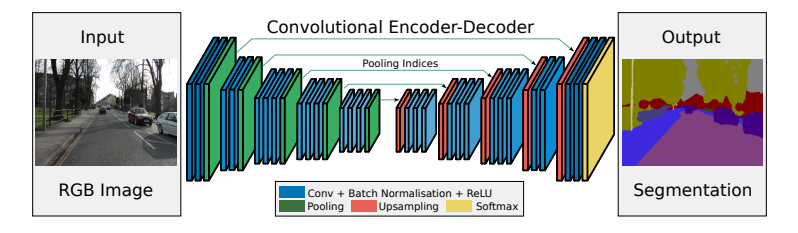
\includegraphics[scale=0.75]{images/segnet.png}
        \caption{SegNet architecture}
        \label{fig:segnet}
    \end{figure}
    
    \item \textbf{DeepLab} \cite{chen2018encoder}: it's primarily a convolutional neural network (CNN) architecture. Unlike the other two networks, it uses features from every convolutional block and then concatenates them to their deconvolutional block. The neural network uses the features from the last convolutional block and upsamples it like the fully convolutional network (FCN). It uses the atrous convolution or dilated convolution method for upsampling. The advantage of atrous convolution is that the computation cost is reduced while capturing more information.
\end{itemize}

Foundation models have also been used for image segmentation, which divides an image into distinct regions or segments. Unlike language models, which are typically based on transformer architectures, foundation models for image segmentation often use convolutional neural networks (CNNs) designed to handle image data.
\begin{itemize}
    \item \textbf{Segment Anything Model (SAM)} \cite{kirillov2023segment}: is considered the first foundation model for image segmentation. 
    SAM is built on the largest segmentation dataset to date, with over 1 billion segmentation masks. 
    It is trained to return a valid segmentation mask for any prompt, where a prompt can be foreground or background points, a rough box or mask, freeform text, or general information indicating what to segment in an image.
    Under the hood, an image encoder produces a one-time embedding for the image, while a lightweight encoder converts any prompt into an embedding vector in real time. 
    These two information sources are combined in a lightweight decoder that predicts segmentation tasks.
\end{itemize}

\begin{figure}[h]
    \centering
    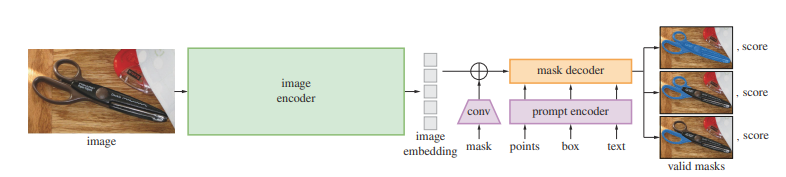
\includegraphics{images/sam.png}
    \caption{Segment Anything Model (SAM) overview.}
    \label{fig:sam}
\end{figure}


\subsubsection*{Limitations of deep learning methods} 
As image segmentation continues to advance, future directions will focus on improving segmentation accuracy, integrating deep learning with traditional techniques, and exploring new applications in various fields. \\Auto-segmentation with the Segment Anything Model (SAM) is a promising direction that can reduce manual intervention and improve accuracy. \\Integration of deep learning with traditional techniques can also help to overcome the limitations of individual techniques and improve overall performance. With ongoing research and development, we can expect image segmentation to continue to make significant contributions to various fields and industries.\\

Of course, deep learning methods have significantly advanced the field of medical image segmentation, but they also have some limitations:
\begin{itemize}
    \item \textbf{Data requirements}: deep methods typically require large amounts of labelled data for training. In the medical field, obtaining such data can be challenging due to privacy issues, the effort required to label medical images, and the need for expert knowledge to provide accurate labels.
    \item \textbf{Computational resources}: training deep learning models can be computationally intensive, requiring powerful hardware and potentially long training times.
    \item \textbf{Generalizability}: while deep learning models can achieve high performance on the data they were trained on, they may not generalize well to new data or different tasks.
    \item \textbf{Segmentation accuracy}: despite the great achievements of medical image segmentation in recent years, medical image segmentation based on deep learning has still encountered difficulties in research. For example, the segmentation accuracy is not high, the number of medical images in the dataset is small and the resolution is low.
    \item \textbf{Clinical requirements}: the inaccurate segmentation results are unable to meet the actual clinical requirements.
\end{itemize}


